\documentclass[overlapped,line,final]{res}

\usepackage[spanish]{babel} % spanish Latex support
\usepackage[utf8]{inputenc} % 
\usepackage{graphicx}       % graphics support
\usepackage[T1,hyphens]{url}
\usepackage[hidelinks,breaklinks=true]{hyperref} %url hyphenation

%----------------------------------------------------------
%----------------------------------------------------------header
\begin{document}

%name
\name{{\Large \bf David Toro Triana}}

\begin{resume}

%-----------------------------------------------personal info, photo

%\begin{minipage}{\linewidth}
	\begin{minipage}{0.5\linewidth}
    		Carrera 15 \# 188-11  \newline 
    		Bogotá D.C., Colombia \newline
    		(+57) 313 255 98 64 \newline
    		{\tt dtorot@opensai.org}
     	%{\tt https://opensai.org} 
	\end{minipage}
%	\begin{minipage}{0.5\linewidth}
%		\begin{center}
%			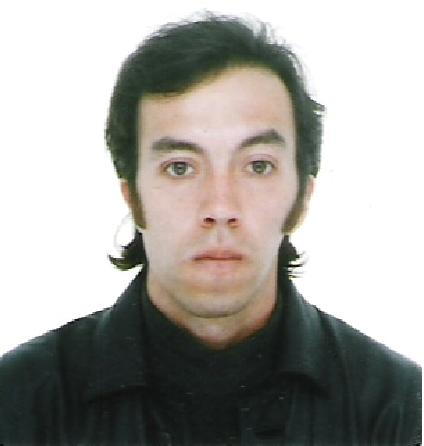
\includegraphics[bb=0 0 100 105, width=30mm,keepaspectratio]{foto.jpeg}
%\begin{center}
%	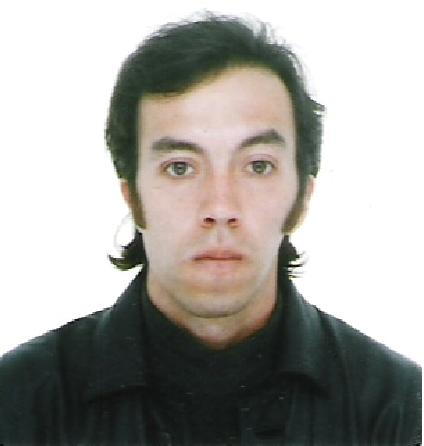
\includegraphics[width=3cm, bb=0 0 305 321]{./foto.jpeg}
%	% foto.jpeg: 424x446 pixel, 100dpi, 10.77x11.33 cm, bb=0 0 305 321
%\end{center}
%		\end{center}
%	\end{minipage}
%\end{minipage}


%----------------------------------------------------Professional Profile 
\vspace{0.5cm}
\section{\sc Professional Profile}
\vspace{0.5cm}
During the last 10 years, I have been working in the field of Web Development and GNU/Linux Systems Administration, thanks to the FLOSS ( {\em Free Libre Open Source Software } ) movement, which allowed me to research, to learn and to contribute to industry and the academy in those fields:

\vspace{2mm}
\begin{itemize}
    \item I have experience in the deployment and administration of services LAMP, in the main GNU/Linux distributions (CentOS-Red Hat-Fedora \& Debian-Ubuntu). 

    \item Also I have worked as Frontend Developer using web standards like HTML5, CSS3 and JavaScript, CSS preprocessors (Bootstrap), using the most popular CMS's and frameworks like Joomla! or Django.

    \item I like to work and explore continuosly game changer platforms like Docker, Kubernets, new app development trends like JAMStack, Progressive Web Apps - PWA or React Native, through debugging, troubleshooting and deploying in the server side.
\end{itemize}
    
I understand that the technology is merely a tool to get organizational goals. From a multicultural environments and goal-oriented leadership, I like to build and maintain productive relationships with clients and colleagues, to gathering, assessing and analysing customer needs, translating business requirements in solution design and effective customer experience.

%-----------------------------------------------------Projects
% \vspace{1cm}
\vspace{0.5cm}
\section{\sc Projects } %-- twixt \location{} & \begin{position}
\vspace{0.5cm}
% -------------------------------------------
\title{\bf Legal Representation
	\newline \em Open Source Academic Initiative (NGO).
	\newline {\tt https://opensai.org} 
}
\employer{\em Legal Rep. (Substitute) – \bf Miguel Ángel González Garzón}
\location{\em (+57) 320 3614052 }
\dates{\bf  January 2013 - 2020 }
\begin{position}
Legal Representation and projects management:

\begin{itemize}
\item Management of Open Source services brief (https://opensai.org/business)
\item Development of pedagogical content and follow-up of the educational process of the \textit{Programa de Fortalecimiento de Capacidades - Formación en animación digital, 2D, 3D, StopMotion y Efectos Especiales ANIMADELAB} (Facultad de Ingeniería, Universidad Nacional de Colombia - 2015 - MinTIC)
\item Learning platform (EdX) for blind people (Facultad de Ingeniería, Universidad Nacional de Colombia, INCI - 2015 )
\item Signing of the cooperation agreement with the Universidad Nacional de Colombia (Facultad de Ingeniería – Octubre 2010)
\item Signing of the cooperation agreement with the Universidad Minuto de Dios – \#OpenLAB (Facultad de Ingeniería – Febrero 2017)
\end{itemize}

\end{position}

% -------------------------------------------
\title{\bf CERI Internationalization Platform
	\newline \em Universidad Distrital Francisco José de Caldas - UDFJC.
	\newline {\tt https://ceri.udistrital.edu.co} 
}
\employer{\em Director – \bf Dr. Alexis Adamy Ortiz Morales }
\location{\em 323 9300 Ext 1007 – Carrera 7 No 40 - 53 Piso 3 }
\dates{\bf  July 2010 – December 2019 }
\begin{position}
Development, support, maintenance of services, utilities, tools and interactive content of the web platform of the \textit {Centro de Relaciones Interinstitucionales - CERI}. It includes Agreements Directory, International Students Aplication System (academic mobility), API integration with the \textit {Universidad Distrital Francisco José de Caldas - UDFJC} academic management system.

The initiative was recognized by the CNA (https://www.cna.gov.co) in 2013, as a best good practices in internacionalization in Colombia, within the framework of high quality accreditation:
\begin{itemize}
\item https://www.cna.gov.co/1741/article-320722.html
\end{itemize}

\end{position}

% -------------------------------------------
\title{\bf Associate Engineer
	\newline \em Tecnologías Xue Ltda (closed).
	\newline {\tt http://xue.com.co} 
}
\employer{\em Legal Representation – \bf Verónica González }
\location{\em (+57) 300 2412225
	\newline Carrera 46 No 93-27 Oficina 101 }
\dates{\bf  Julio 2006 – Febrero 2008 }
\begin{position}
Integration and implementation of security biometric solutions, and corporate open source solutions, using the classical methodologies of system and software engineering.
\end{position}

%-----------------------------------------------------Proyectos en construcción
\newpage
\opening

%-------------------------------------------------------Educación
%\newpage
%\opening
\section{\sc Education}
\vspace{0.5cm}
Systems Engineer (Ingeniero de Sistemas)
\newline Graduation Project \textit{SISTEMA DE RENDER DISTRIBUIDO TIPO CLUSTER, INTEGRABLE COMO RECURSO A UN ENTORNO DE COMPUTACION GRID}
\newline Universidad Distrital Francisco José de Caldas - UDFJC

\vspace{0.25cm}

%------------------------------------------------------Areas de trabajo
\section{\sc Special skills and knowledge}
\vspace{0.5cm}
\begin{itemize}
	\item Configuration and administration of the operating systems GNU/Linux (Debian, CentOS), with the related aplications and services (Apache, MySQL, Nginx)
	\item Open Source applications cloud deployment (Linode, Azure, AWS) 
	\item Customization and administration of web Content Management Systems - CMS's (Wordpress, Joomla!, Drupal), Learning Management Systems - LMS's (Moodle, EdX)
	\item Basic development skills in C/C++, Python (Django)
 	\item Content creation using open source design and editing tools (Gimp, Inkscape, OpenShot)
\end{itemize}

%------------------------------------------------------Areas de trabajo
\section{\sc Areas of interest and research}
\vspace{0.5cm}
\begin{itemize}
	\item Computer Graphics / Scientific Computing
	\begin{itemize}
	 \item Configuration and Administration of the Terascale Open-source Resource and QUEue Manager TORQUE ({\url https://github.com/adaptivecomputing/torque}) and Globus Toolkit ({\url https://toolkit.globus.org/}) at the CECAD ({\url https://tinyurl.com/y5ksh6by}) in render OpenGL 3D imagery and grid computing (2011-2014)
	 \begin{itemize}
	  \item 64 nodes (16 physicals)
	  \item 32 Tb RAM
	  \item shared storage in S.A.N.
	 \end{itemize}
	 \item OpenCL, MPI (Message Passing Interface) in C/C++ and Python, over a Beowulf MOSIX or Pelican HPC cluster, to support galaxy spectral analysis in the COMPUCIE team ({\url https://tinyurl.com/y3knf9b7}) 
	 \item HPC provisioning over Azure CycleCloud (entry level by institutional budget)
	\end{itemize}
	\item Infrastructure Orchestration and services using Docker, Kubernetes (AKS, OpenShift)
	\item The \LaTeX documentation system	
    \item Good engineering practices, ethical hacking
	\item Open licensing and innovation support
    \item New technologies social aplication:
    \begin{itemize}
		\item New education and social, digital inclusion models
	    \item Alternative models of economic self-sufficiency, cultural identity, civil society and democracy
	    \item Food self-sufficiency, ecology, sustainability (permaculture)
    \end{itemize}

	
\end{itemize}

\newpage
\opening
\section{\sc Personal References}

Omaira Tovar Ruiz \newline
Instituto Colombiano del Sistema Nervioso Clínica – Monserrat\newline
Calle 134 \# 17 – 71 \newline
2596000 Extensión 6009\newline
\url{omairatovar@gmail.com} \newline
Information Science Professional, Librarianship and Archivist (Profesional en Ciencias de la Información, Bibliotecología y Archivista)

Olman Yair Vasquez\newline
MINCIVIL\newline
316 8089525\newline
\url{ovasquez@mincivil.com}\newline
Systems Engineer (Ingeniero de Sistemas, Especialista en Gestión de Proyectos)

\vspace{\fill}
\begin{minipage}{1.0\linewidth}
\begin{center}	
	
\includegraphics[width=7cm,bb=0 0 1147 1147]{./qr.png}
	%
\includegraphics[width=4cm,bb=0 0 598 417]{./sign.jpeg}
	% firma.jpeg: 598x417 pixel, 72dpi, 21.10x14.71 cm, bb=0 0 598 417
\end{center}
\end{minipage}


\vspace{\fill}\ \newline
{\tiny \rm $ $Powered by \LaTeX $ $ }
{\tiny \rm $ $Junio 2017$ $ }
{\tiny \rm $ $Nemqueteba Currículum Versión 0.02 $ $ }

\end{resume}
\end{document}

%---------------------------------------------------------------------
%---------------------------------------------------------------------fin documento
